\documentclass[tikz,border=8pt]{standalone}
\usetikzlibrary{arrows.meta,positioning,fit,backgrounds,calc}

\begin{document}
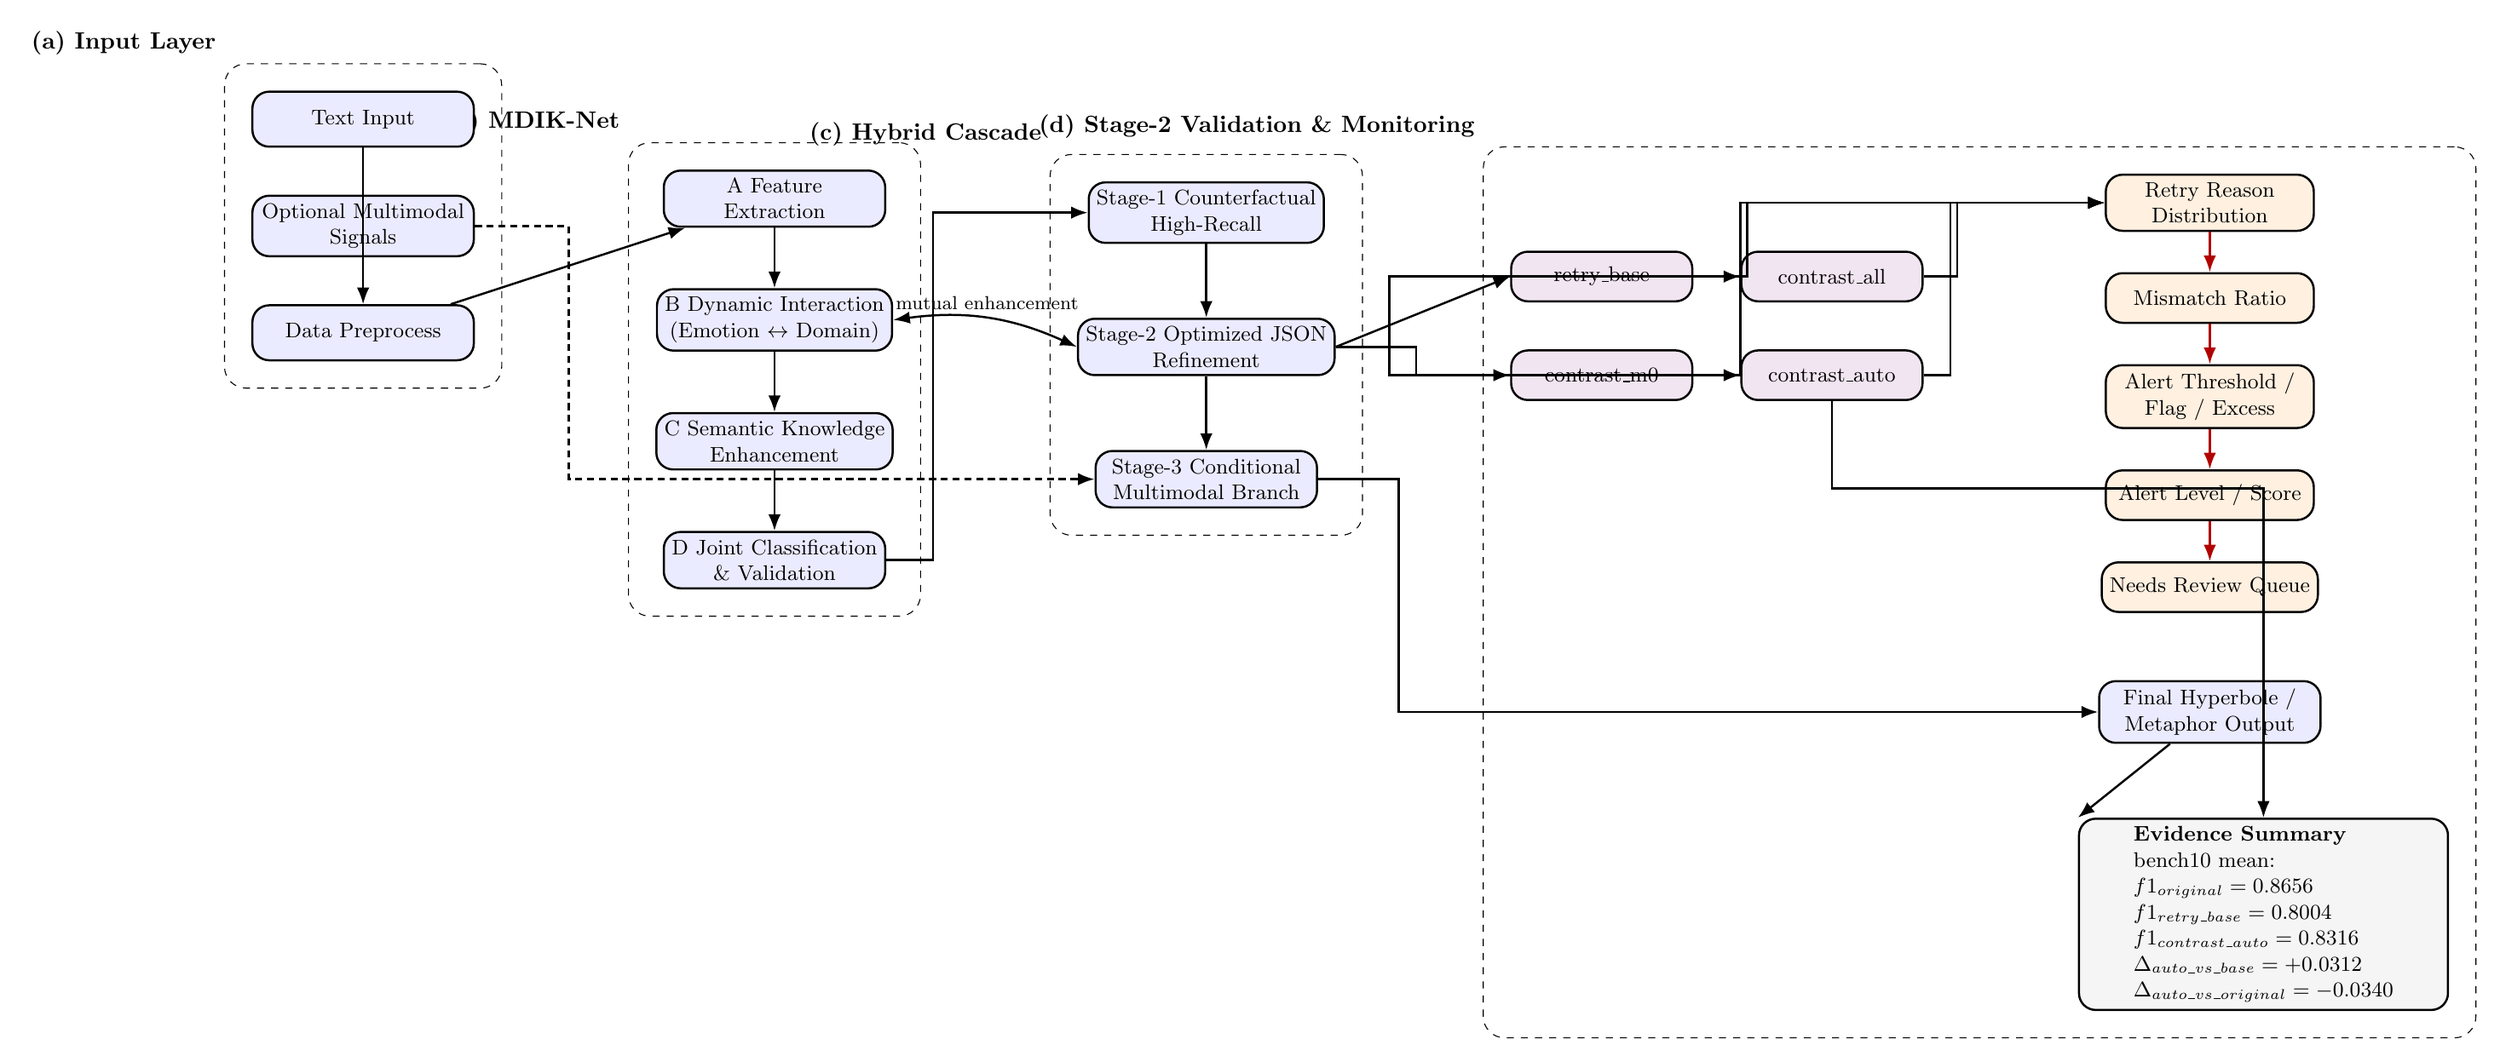
\begin{tikzpicture}[
  font=\small,
  >={Latex[length=2.5mm,width=1.8mm]},
  line width=0.9pt,
  module/.style={draw,rounded corners=2.5mm,minimum width=33mm,minimum height=8.2mm,align=center,fill=blue!8},
  branch/.style={draw,rounded corners=2.5mm,minimum width=27mm,minimum height=7.4mm,align=center,fill=violet!10},
  monitor/.style={draw,rounded corners=2.5mm,minimum width=31mm,minimum height=7.4mm,align=center,fill=orange!12},
  evidence/.style={draw,rounded corners=2.5mm,minimum width=55mm,minimum height=23mm,align=left,fill=gray!8},
  panel/.style={draw,dashed,rounded corners=3.2mm,inner sep=4mm},
  mainflow/.style={-Latex},
  auxflow/.style={-Latex,densely dashed},
  bidiflow/.style={<->,bend left=16},
  alertflow/.style={-Latex,draw=red!70!black}
]

% ===== Input Layer =====
\node[module] (text) {Text Input};
\node[module,below=7mm of text] (multi) {Optional Multimodal\\Signals};
\node[module,below=7mm of multi] (prep) {Data Preprocess};

% ===== MDIK-Net =====
\node[module,right=28mm of prep,yshift=20mm] (A) {A Feature\\Extraction};
\node[module,below=9mm of A] (B) {B Dynamic Interaction\\(Emotion $\leftrightarrow$ Domain)};
\node[module,below=9mm of B] (C) {C Semantic Knowledge\\Enhancement};
\node[module,below=9mm of C] (D) {D Joint Classification\\\& Validation};

% ===== Hybrid Cascade =====
\node[module,right=29mm of B,yshift=16mm] (S1) {Stage-1 Counterfactual\\High-Recall};
\node[module,below=11mm of S1] (S2) {Stage-2 Optimized JSON\\Refinement};
\node[module,below=11mm of S2] (S3) {Stage-3 Conditional\\Multimodal Branch};

% ===== Stage-2 Branches =====
\node[branch,right=26mm of S2,yshift=10.5mm] (rb) {retry\_base};
\node[branch,right=7mm of rb] (ca) {contrast\_all};
\node[branch,below=7mm of rb] (cm) {contrast\_m0};
\node[branch,right=7mm of cm] (cu) {contrast\_auto};

% ===== Monitoring =====
\node[monitor,right=27mm of ca,yshift=11mm] (rr) {Retry Reason\\Distribution};
\node[monitor,below=6mm of rr] (mr) {Mismatch Ratio};
\node[monitor,below=6mm of mr] (af) {Alert Threshold /\\Flag / Excess};
\node[monitor,below=6mm of af] (ls) {Alert Level / Score};
\node[monitor,below=6mm of ls] (nr) {Needs Review Queue};
\node[module,below=10mm of nr] (out) {Final Hyperbole /\\Metaphor Output};

% ===== Evidence =====
\node[evidence,below=11mm of out,xshift=8mm] (ev) {
\textbf{Evidence Summary}\\
bench10 mean: \\
$f1_{original}=0.8656$\\
$f1_{retry\_base}=0.8004$\\
$f1_{contrast\_auto}=0.8316$\\
$\Delta_{auto\_vs\_base}=+0.0312$\\
$\Delta_{auto\_vs\_original}=-0.0340$
};

% ===== Main Flow =====
\draw[mainflow] (text) -- (prep);
\draw[mainflow] (prep) -- (A);
\draw[mainflow] (A) -- (B);
\draw[mainflow] (B) -- (C);
\draw[mainflow] (C) -- (D);
\draw[mainflow] (D.east) -- ++(7mm,0) |- (S1.west);
\draw[mainflow] (S1) -- (S2);
\draw[mainflow] (S2) -- (S3);
\draw[mainflow] (S3.east) -- ++(12mm,0) |- (out.west);

% ===== Auxiliary / Branch =====
\draw[auxflow] (multi.east) -- ++(14mm,0) |- (S3.west);
\draw[mainflow] (S2.east) -- (rb.west);
\draw[mainflow] (S2.east) -- ++(8mm,0) |- (ca.west);
\draw[mainflow] (S2.east) -- ++(8mm,0) |- (cm.west);
\draw[mainflow] (S2.east) -- ++(12mm,0) |- (cu.west);

% ===== Monitoring Chain =====
\draw[mainflow] (rb.east) -- ++(8mm,0) |- (rr.west);
\draw[mainflow] (ca.east) -- ++(5mm,0) |- (rr.west);
\draw[mainflow] (cm.east) -- ++(7mm,0) |- (rr.west);
\draw[mainflow] (cu.east) -- ++(4mm,0) |- (rr.west);
\draw[alertflow] (rr) -- (mr);
\draw[alertflow] (mr) -- (af);
\draw[alertflow] (af) -- (ls);
\draw[alertflow] (ls) -- (nr);
\draw[mainflow] (out) -- (ev.north west);
\draw[mainflow] (cu.south) -- ++(0,-13mm) -| (ev.north);

% ===== Bidirectional Hint =====
\draw[bidiflow] (B.east) to node[midway,above,font=\footnotesize]{mutual enhancement} (S2.west);

% ===== Panels =====
\begin{scope}[on background layer]
  \node[panel,fit=(text)(multi)(prep),label={[font=\bfseries]north west:(a) Input Layer}] {};
  \node[panel,fit=(A)(B)(C)(D),label={[font=\bfseries]north west:(b) MDIK-Net}] {};
  \node[panel,fit=(S1)(S2)(S3),label={[font=\bfseries]north west:(c) Hybrid Cascade}] {};
  \node[panel,fit=(rb)(ca)(cm)(cu)(rr)(mr)(af)(ls)(nr)(out)(ev),label={[font=\bfseries]north west:(d) Stage-2 Validation \& Monitoring}] {};
\end{scope}

\end{tikzpicture}
\end{document}
